\subsection{Measurement- and perturbation-layer visibility: LINCS L1000 via iLINCS (fourth invisibility axis; connectivity pilot negative)}
\label{sec:ilincs}
All three prior druggability audits asked whether the pharmacopeia
\emph{engages} the gated antigens. The LINCS L1000 resource (queried through
the iLINCS API, \texttt{results/ilincs\_summary.json}) answers a prior
question: whether the world's largest perturbational transcriptomics dataset
can even \emph{see} these genes. It cannot. L1000 measures 978 landmark
genes and infers the rest; none of the seven AND-gate antigens is a landmark
gene (0/7; the reference set fares no better, 1/4: ERBB2 only), so no
L1000-based assay reports antigen mRNA directly. The perturbation layer is
nearly as blind: \textbf{5 of 7 antigens have no consensus knockdown
signature at all} in the 36,692-signature CGS library (CA12: 12 and
SLC39A6: 7 across the nine core cell lines; CLDN18, MSLN, CA9, CLDN6, PSCA:
zero). This is not gate-selection bias: the full 99-gene gated set is as
landmark-visible as the random surfaceome (7/99\ versus
5/98\ genes, Fisher $p=0.767$) and modestly \emph{better} covered by
knockdowns (30/99\ versus 17/NBG, $p=0.044$), so the antigens'
invisibility is their own property, not an artifact of how the gate was
built. Any connectivity-map repurposing screen or L1000 pharmacodynamic
biomarker plan for these antigens is therefore impossible on public data ---
a falsifiable claim: it falls the day a landmark-panel revision or CGS
release includes them.

The knockdown signatures that do exist carry gene-specific signal:
within-gene cross-cell-line agreement (median Spearman
$\rho=0.175$, $n=153$ pairs) exceeds between-gene agreement
($\rho=0.058$, $n=312$; Mann--Whitney $p=7.9e-14$). The single
ERBB2 overexpression signature, however, does not anticorrelate with the
ERBB2 knockdowns ($\rho=0.002$; $n=1$ OE, underpowered). A connectivity
pilot against the project's own pharmacopeia (198 GDSC compounds, 1,374\
exemplar compound signatures) then \emph{fails its positive control}:
ERBB2 knockdown connectivity should rank EGFR/HER2 inhibitors on top, but
only 1 of the top 20 mimics is an EGFR-class drug (16/198 background,
Fisher $p=1.0$; top ranks are LDN-193189, Piperlongumine, AT7867, MG-132, PAC-1, Omipalisib, JW-7-24-1, Palbociclib). CGS-consensus connectivity at
landmark resolution therefore does not recover known pharmacology here, and
the CA12 and SLC39A6 mimic tables (top by rank: AZD7762 ($\rho$=0.135), Y-39983 ($\rho$=0.117), GSK1070916 ($\rho$=0.105), Veliparib ($\rho$=0.105), Ruxolitinib ($\rho$=0.1); Ibrutinib ($\rho$=0.5), AT7867 ($\rho$=0.482), XMD15-27 ($\rho$=0.451), Bicalutamide ($\rho$=0.438), Foretinib ($\rho$=0.427)) are
reported as data only, not as repurposing hypotheses; no GDSC pathway is
enriched among the top-30 mimics after Benjamini--Hochberg correction
(smallest $q$: CA12 0.29, SLC39A6 0.12). The SLC39A6 connectivity
distribution is globally shifted positive (median $\rho=0.160$ versus
CA12 0.015), consistent with a proliferation-dominated knockdown
signature; we do not interpret it further.

\begin{figure}[h]\centering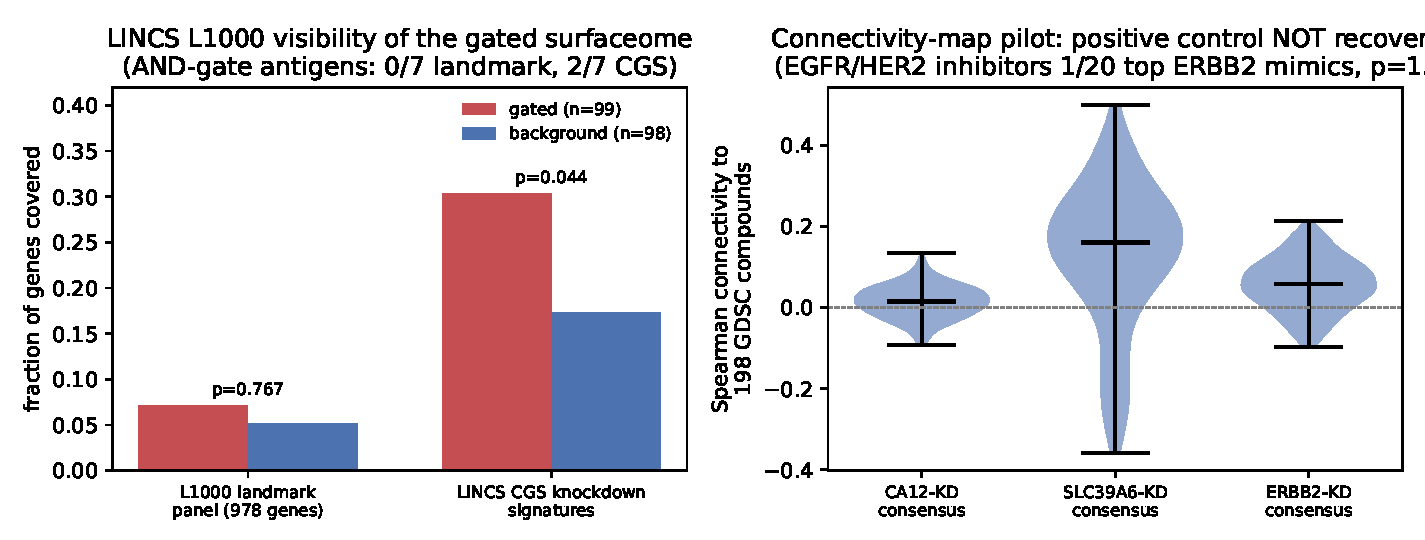
\includegraphics[width=0.98\linewidth]{figs/fig_ilincs.pdf}
\caption{Left: gated versus background coverage in the L1000 landmark panel and CGS knockdown library. Right: compound-connectivity distributions to the CA12, SLC39A6 and ERBB2 knockdown consensuses across 198 GDSC compounds.}
\end{figure}
